\documentclass[12pt]{article}

\usepackage[a4paper,margin=2cm]{geometry}
\usepackage{amsmath, amssymb, amsthm, amsfonts, tikz, algpseudocode}
\usepackage[plain]{algorithm}
\usepackage[framemethod=TikZ]{mdframed}
\definecolor{newblue}{rgb}{0.2,0.2,0.6}
\usepackage{caption}
\usepackage{graphicx}
\usepackage{float}
\usepackage{listings}
\usepackage{color}
\usepackage[colorlinks,allcolors=newblue]{hyperref}
\usepackage{listings}
\lstset{
    language=R,
    basicstyle=\scriptsize\ttfamily,
    commentstyle=\ttfamily\color{gray},
    numbers=left,
    numberstyle=\ttfamily\color{gray}\footnotesize,
    stepnumber=1,
    numbersep=5pt,
    backgroundcolor=\color{white},
    showspaces=false,
    showstringspaces=false,
    showtabs=false,
    frame=single,
    tabsize=2,
    captionpos=b,
    breaklines=true,
    breakatwhitespace=false,
    title=\ttfamily\lstname,
    escapeinside={},
    keywordstyle={},
    morekeywords={}
}

\theoremstyle{plain}
\newtheorem*{theorem}{Theorem}
\newtheorem*{lemma}{Lemma}
\newtheorem*{claim}{Claim}
\newtheorem*{definition}{Definition}
\newtheorem*{corollary}{Corollary}
\newtheorem*{remark}{Remark}
\newtheorem*{proposition}{Proposition}
\DeclareMathOperator*{\argmin}{arg\,min}
\DeclareMathOperator*{\eig}{eig}

\newcommand{\handout}[5]{
   \renewcommand{\thepage}{#1-\arabic{page}}
   \noindent
   \begin{center}
   \framebox{
      \vbox{
    \hbox to 5.78in { {\bf MATH 690: Topics in Probablity Theory} \hfill #2 }
       \vspace{4mm}
       \hbox to 5.78in { {\Large \hfill #5  \hfill} }
       \vspace{2mm}
       \hbox to 5.78in { {\it #3 \hfill #4} }
      }
   }
   \end{center}
   \vspace*{4mm}
}

\renewcommand{\paragraph}[1]{\medskip \noindent {\bf #1.}}

\newcommand{\lecture}[4]{\handout{#1}{#2}{Lecturer: #3}{Scribes: #4}{#1}}

%%%% TITLE

\title{Math 690: Topics in Data Analysis and Computation \\
Lecture notes for October 3, 2017}
\date{}

\author{Scribed by Dev Dabke and Andrew Cho}

%%%%%% FOUND AT
% https://texblog.org/2015/09/30/fancy-boxes-for-theorem-lemma-and-proof-with-mdframed/

%%%%%%%%%%%%%%%%%%%%%%%%%%%%%%
%Theorem
\newcounter{theo}[section]\setcounter{theo}{0}
\renewcommand{\thetheo}{\arabic{section}.\arabic{theo}}
\newenvironment{theo}[2][]{%
\refstepcounter{theo}%
\ifstrempty{#1}%
{\mdfsetup{%
frametitle={%
\tikz[baseline=(current bounding box.east),outer sep=0pt]
\node[anchor=east,rectangle,fill=blue!20]
{\strut Theorem~\thetheo};}}
}%
{\mdfsetup{%
frametitle={%
\tikz[baseline=(current bounding box.east),outer sep=0pt]
\node[anchor=east,rectangle,fill=blue!20]
{\strut Theorem~\thetheo:~#1};}}%
}%
\mdfsetup{innertopmargin=5pt,innerbottommargin=10pt,linecolor=blue!20,%
linewidth=2pt,topline=true,%
frametitleaboveskip=\dimexpr-\ht\strutbox\relax
}
\begin{mdframed}[]\relax%
\label{#2}}{\end{mdframed}}

%%%%%%%%%%%%%%%%%%%%%%%%%%%%%%
%Lemma

\newcounter{lem}[section]\setcounter{lem}{0}
\renewcommand{\thelem}{\arabic{section}.\arabic{lem}}
\newenvironment{lem}[2][]{%
\refstepcounter{lem}%
\ifstrempty{#1}%
{\mdfsetup{%
frametitle={%
\tikz[baseline=(current bounding box.east),outer sep=0pt]
\node[anchor=east,rectangle,fill=green!20]
{\strut Lemma~\thelem};}}
}%
{\mdfsetup{%
frametitle={%
\tikz[baseline=(current bounding box.east),outer sep=0pt]
\node[anchor=east,rectangle,fill=green!20]
{\strut Lemma~\thetheo:~#1};}}%
}%
\mdfsetup{innertopmargin=5pt,innerbottommargin=10pt,linecolor=green!20,%
linewidth=2pt,topline=true,%
frametitleaboveskip=\dimexpr-\ht\strutbox\relax
}
\begin{mdframed}[]\relax%
\label{#2}}{\end{mdframed}}

%%%%%%%%%%%%%%%%%%%%%%%%%%%%%%
%Proof

\newcounter{prf}[section]\setcounter{prf}{0}
\renewcommand{\theprf}{\arabic{section}.\arabic{prf}}
\newenvironment{prf}[2][]{%
\refstepcounter{prf}%
\ifstrempty{#1}%
{\mdfsetup{%
frametitle={%
\tikz[baseline=(current bounding box.east),outer sep=0pt]
\node[anchor=east,rectangle,fill=red!20]
{\strut Proof~\theprf};}}
}%
{\mdfsetup{%
frametitle={%
\tikz[baseline=(current bounding box.east),outer sep=0pt]
\node[anchor=east,rectangle,fill=red!20]
{\strut Proof~\thetheo:~#1};}}%
}%
\mdfsetup{innertopmargin=5pt,innerbottommargin=10pt,linecolor=red!20,%
linewidth=2pt,topline=true,%
frametitleaboveskip=\dimexpr-\ht\strutbox\relax
}
\begin{mdframed}[]\relax%
\label{#2}}{\end{mdframed}}

%%%%%%%%%%%%%%%%%%%%%%%%%%%%%%
%Remark
\newcounter{rmk}[section]\setcounter{rmk}{0}
\renewcommand{\thermk}{\arabic{section}.\arabic{rmk}}
\newenvironment{rmk}[2][]{%
\refstepcounter{rmk}%
\ifstrempty{#1}%
{\mdfsetup{%
frametitle={%
\tikz[baseline=(current bounding box.east),outer sep=0pt]
\node[anchor=east,rectangle,fill=yellow!50]
{\strut Remark~\thermk};}}
}%
{\mdfsetup{%
frametitle={%
\tikz[baseline=(current bounding box.east),outer sep=0pt]
\node[anchor=east,rectangle,fill=yellow!50]
{\strut Remark~\thermk:~#1};}}%
}%
\mdfsetup{innertopmargin=5pt,innerbottommargin=10pt,linecolor=yellow!50,%
linewidth=2pt,topline=true,%
frametitleaboveskip=\dimexpr-\ht\strutbox\relax
}
\begin{mdframed}[]\relax%
\label{#2}}{\end{mdframed}}

%%%%%%%%%%%%%%%%%%%%%%%%%%%%%%
%Definiton
\newcounter{dfn}[section]\setcounter{dfn}{0}
\renewcommand{\thedfn}{\arabic{section}.\arabic{dfn}}
\newenvironment{dfn}[2][]{%
\refstepcounter{dfn}%
\ifstrempty{#1}%
{\mdfsetup{%
frametitle={%
\tikz[baseline=(current bounding box.east),outer sep=0pt]
\node[anchor=east,rectangle,fill=purple!20]
{\strut Definition~\thedfn};}}
}%
{\mdfsetup{%
frametitle={%
\tikz[baseline=(current bounding box.east),outer sep=0pt]
\node[anchor=east,rectangle,fill=purple!20]
{\strut Definition~\thedfn:~#1};}}%
}%
\mdfsetup{innertopmargin=5pt,innerbottommargin=10pt,linecolor=purple!20,%
linewidth=2pt,topline=true,%
frametitleaboveskip=\dimexpr-\ht\strutbox\relax
}
\begin{mdframed}[]\relax%
\label{#2}}{\end{mdframed}}


\begin{document}
\lecture{Clustering}{October 3, 2017}{Xiuyuan Cheng}{Dev Dabke and Andrew Cho}

\section{Introduction}
The lecture covered
\begin{itemize}
	\item A discussion of KK10 paper on the consistency of Lloyd's k-means algorithm
	\item An introduction to Spectral Clustering
\end{itemize}

\section{k-means clustering}
\label{sec:kmeans}

\subsection{Lloyd's algorithm}
\label{subsec: lloyd}

Recall Lloyd's algorithm from last lecture that given some data points as input $ \{ x_i \}^n_{i = 1} $, we want to search for $ k $ clusters $ C = \{ C_1, \ldots, C_k \} $ with ``centers'' $ \mu = \{ \mu_1, \ldots, \mu_k \} $.
\\ \\
\begin{dfn}[Objective Functions]{dfn:objective}
Depending on our constraints, also recall we can choose different objective functions and have different interpretations of what these clusters represent.
\begin{align*}
  \min_{C, \mu} & \sum_{l = 1}^k \sum_{i \in C_{l}} \| x_i - \mu_{l} \|_2^2 & \text{k means} \\
  \min_{C, \mu} & \sum_{l = 1}^k \sum_{i \in C_{l}} \| x_i - \mu_{l} \|_{1} & \text{k medians} \\
  \min_{C, \mu} & \sum_{l = 1}^k \sum_{i \in C_{l}} \| x_i - \mu_{l} \|_2 & \text{$ L_2 $ - $ L_1 $ norm}
\end{align*}
\end{dfn}
We can either choose initial seeds by randomly selecting k points or by singular value decomposition (SVD). Ultimately, we are interested in knowing if these results are \textit{consistent}.
Can these seeding methods lead to the true centroids?

\subsection{Strong Law of Large Numbers}
\label{subsec:slln}
\begin{dfn}[Loss]{dfn:loss}
	\[
	\mathcal{L}_n (\mu) = \int \| x - \mu \|^2 d P_n(x)
	\]
	where
	\[
	d P_n (x) = \frac{1}{n} \sum_{i = 1}^n \delta_{x_i} (x) dx
	\]
	which is the empirical measure of the data.
\end{dfn}
\begin{dfn}[Element-Set Norm]{dfn:norm}
	Where $ A = \{ a_1, \ldots, a_n \} $ for all $ x \in \mathbb{R} $, we define $ \| x - A \| $ to be
	\[
	\| x - A \| = \min_{1 \leq i \leq n} \| x - a_i \|
	\]
\end{dfn}
\begin{theo}[Strong Law of Large Numbers]{theo:slln}
	As $ n \to \infty $
	\begin{align*}
		\mathcal{L} (\mu) &= \int \| x - \mu \|^2 dP(x) \\
		\min_{\mu} \mathcal{L}_n (\mu) &\to \min_{\mu} \mathcal{L} (\mu)
	\end{align*}
\end{theo}

\subsection{Consistency of Lloyd}
\label{subsec:consistency}
If we satisfy some requirements of ``separation,'' then we can provide some bound for misclassification, assuming some true centroid partition.~\cite{kumar-2010}
$ \| \mu^{*}_{k} - \mu^{*}_{l} \| $ if $ k \neq l $ needs to be bigger than a gap $ \Delta_{kl} $.
\\ \\
\[
\Delta_{kl} > c \frac{\sigma_l}{\sqrt{w_{min}}} \hspace{1cm} w_{min} = \min_{l} \frac{|C_l^{*}|}{n}
\]
$w_{min}$ denotes proportions of points in cluster $l$. Letting $ \sigma_k^2 $ be the variance of the data in the $ k^{th} $ cluster and if we can assume that $ \sigma_k \approx \sigma_l $, then we know that misclassification error from SVD initialization occurs less than some $ \epsilon * n $ with high probability.

\subsection{In Practice}
\label{subsec:inpractice}

There are some practical considerations for k-means.
\begin{enumerate}
  \item What is $ k $?
  \item How to choose an initial seed
  \item Some cases of k-means fails
  \begin{enumerate}
    \item $ \sigma_k $ might be too large compared to separation
    \item Clusters might be too small (i.e.\ cluster sizes may not be balanced)
    \item Cluster might be convex and piecewise can't do concave (Voronoi)
  \end{enumerate}
\end{enumerate}

\section{Spectral clustering}
\label{sec:spectral}

\subsection{Graph Laplacian}

Given some data $ \{ x_i \}_{i = 1}^n $ and $ k $, we want to
\begin{enumerate}
  \item Build positive-definite, symmetric affinity matrix $ W_{n \times n} $ by $ k $ nearest neighbors, $ \epsilon $ - neighbor, or the Gaussian kernel $ W_{ij} = e^{- \frac{\| x_i - x_j \|^2}{\epsilon}} $.
  \item Consider the eigenvalue decomposition of the graph Laplacian $ \mathcal{L} $.
  Note that
  \begin{align*}
    L_{un} &= D - W  & \text{Unnormalized} \\
    L_{rw} &= D^{-1} (D - W) & \text{Shi-Malik '00} \\
    L_{sym} &= I - D^{-1/2} W D^{-1/2} & \text{Ng-Jordan-Weiss '02}
  \end{align*}
  \item Apply k means to $ \Psi = [\varphi_i, \ldots, \varphi_k]_{n \times k} $ and denote $ y_i $ as the $ i^{th} $ row of $ \Psi $.
\end{enumerate}

\begin{rmk}[Thresholding]{rmk:truncation}
  If $ k = 2$, you can use thresholding because the first eigenvalue is constant. Thus, you can use sign($\Psi_2$) to indicate clustering.
\end{rmk}

\begin{dfn}[Connected Components]{dfn:connected-components}

Let $ \mathcal{G} = (V, E) $ such that on each edge $ (i, j) \in \mathcal{G} $ that $ w_{ij} > 0 $.
If node $ i $ is connected to node $ j $, there is a path from $ i $ to $ j $.
So then, set $ A $ is a connected component if every pair of $ i $ and $ j $ is connected and $ A $ is the maximum set that satisfies this condition to preserve connectivity.

\end{dfn}

\begin{theo}[Eigenspace of $ \lambda = 0 $ of $\mathcal{L}$]{theo:eigenspace}

Suppose the graph has $ k $ connected components $ A_{1}, \ldots, A_{k} $.
Then the eigenspace of $ \lambda = 0 $ of $ \dim{k} $ is spanned by
\[
\{ \mathbf{1}_{A_{1}}, \ldots, \mathbf{1}_{A_{k}} \}
\]
where
\[
\mathbf{1}_{A_{i}} (i) =
\begin{cases}
  1 & i \in A \\
  0 & \text{otherwise}
\end{cases}
\]

\end{theo}

\begin{prf}[Eigenspace of $ \lambda = 0 $ of $\mathcal{L}$, Theorem~\ref{theo:eigenspace}]
	Suppose $\mathbf{f}$ is an eigenvector with  $\lambda = 0$.
  So $\mathcal{L}\textbf{f} = \textbf{0}$ and $\textbf{f}^T\mathcal{L}\textbf{f} = \textbf{0}$.
  We also know $\textbf{f}^T\mathcal{L}\textbf{f} = \textbf{0} = \frac{1}{2} \sum_{(i,j)}w_{i,j}(f_i-f_j)^2$ and $\textbf{f}^T\mathcal{L}\textbf{f} = \textbf{0} \Leftrightarrow f_i=f_j$ whenever $w_{i,j} > 0$.
  Thus, $\textbf{f}$ is a piecewise constant in each of the connected components.
  Meanwhile, for each $v \in$ span $\{\mathbf{1}_{A_{1}}, \ldots, \mathbf{1}_{A_{k}} \}, \mathbf{v}^T \mathcal{L} \mathbf{v} = \mathbf{0}$.
\end{prf}
\textbf{Exercise}
\begin{itemize}
	\item Does this generalize to $\mathcal{L}_{rw}$ and $\mathcal{L}_{sym}$?
	\item What about consistency of spectral clustering?
\end{itemize}

\section{Applications}

\subsection{Spectral vs. k-means Clustering}

When should we use spectral clustering and when should we use $ k $-means clustering?
One prototypical example is with spirals.
$ k $-means excels when the clusters are assumed to be dense point clouds separated from other dense point clouds.
Spectral clustering works well where clusters may have many points with small local distances (with some metric), i.e.\ concentric circles.
\\ \\
To analyze this situation, we can use \texttt{R} to study this behavior.
\lstinputlisting[language=R]{sc_kmeans_example.R}

\subsection{Using k-means on Images}
We can also use $ k $-means to compress an image.
\lstinputlisting[language=R]{kmeans_compression_example.R}
We can, as an example, compress the Raccoon image in Figure~\ref{fig:raccoon}.
\begin{figure}[H]
  \captionsetup{width=0.8\textwidth}
  \centering
  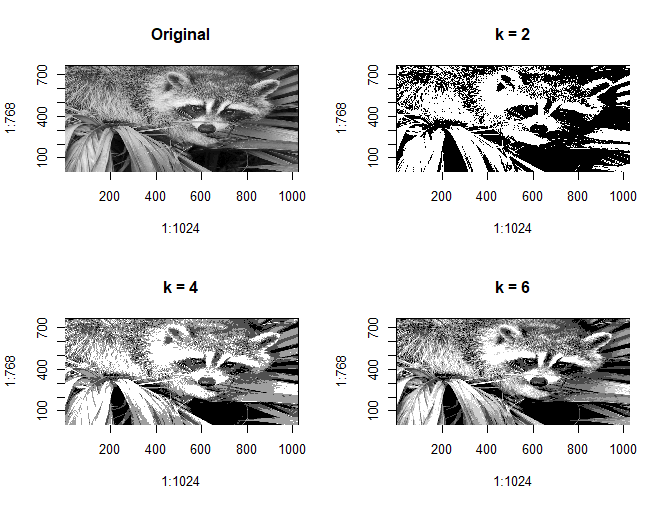
\includegraphics[width=\textwidth]{raccoon}
  \caption{
      A black and white image of a raccoon.
  }
  \label{fig:raccoon}
\end{figure}

\subsection{Basketball Position Data Analysis}

Spectral clustering can also be used with basketball position data.


\bibliography{clustering}{}
\bibliographystyle{alpha}

\end{document}
